\documentclass[aspectratio=169]{beamer}

\mode<presentation>
{
  \usetheme{default}
  \usecolortheme{default}
  \usefonttheme{default}
  \setbeamertemplate{navigation symbols}{}
  \setbeamertemplate{caption}[numbered]
  \setbeamertemplate{footline}[frame number]  % or "page number"
  \setbeamercolor{frametitle}{fg=white}
  \setbeamercolor{footline}{fg=black}
} 

\usepackage[english]{babel}
\usepackage[utf8x]{inputenc}
\usepackage{tikz}
\usepackage{courier}
\usepackage{array}
\usepackage{bold-extra}
\usepackage{minted}
\usepackage[thicklines]{cancel}
\usepackage{booktabs}

\xdefinecolor{dianablue}{rgb}{0.18,0.24,0.31}
\xdefinecolor{darkblue}{rgb}{0.1,0.1,0.7}
\xdefinecolor{darkgreen}{rgb}{0,0.5,0}
\xdefinecolor{darkgrey}{rgb}{0.35,0.35,0.35}
\xdefinecolor{darkorange}{rgb}{0.8,0.5,0}
\xdefinecolor{darkred}{rgb}{0.7,0,0}
\definecolor{darkgreen}{rgb}{0,0.6,0}
\definecolor{mauve}{rgb}{0.58,0,0.82}

\title[2018-02-21-rootio-parquet]{Parquet data format performance}
\author{Jim Pivarski}
\institute{Princeton University -- DIANA-HEP}
\date{February 21, 2018}

\begin{document}

\logo{\pgfputat{\pgfxy(0.11, 7.4)}{\pgfbox[right,base]{\tikz{\filldraw[fill=dianablue, draw=none] (0 cm, 0 cm) rectangle (50 cm, 1 cm);}\mbox{\hspace{-8 cm}
\includegraphics[height=1 cm]{princeton-logo-long.png}
\includegraphics[height=1 cm]{diana-hep-logo-long.png}}}}}

\begin{frame}
  \titlepage
\end{frame}

\logo{\pgfputat{\pgfxy(0.11, 7.4)}{\pgfbox[right,base]{\tikz{\filldraw[fill=dianablue, draw=none] (0 cm, 0 cm) rectangle (50 cm, 1 cm);}\mbox{\hspace{-8 cm}
\includegraphics[height=1 cm]{princeton-logo.png}
\includegraphics[height=1 cm]{diana-hep-logo.png}}}}}

% Uncomment these lines for an automatically generated outline.
%\begin{frame}{Outline}
%  \tableofcontents
%\end{frame}

% START START START START START START START START START START START START START

\begin{frame}{First slide}
\vspace{0.5 cm}
HERE
\end{frame}

\begin{frame}{So-called ``uncompressed'' Parquet is tighter, but gzip is the same}
\vspace{-0.1 cm}
\begin{columns}
\column{0.26\linewidth}
\begin{center}
ROOT uncompressed

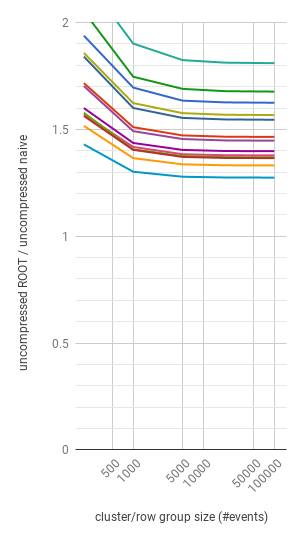
\includegraphics[width=\linewidth]{root-none.png}
\end{center}
\column{0.26\linewidth}
\begin{center}
Parquet uncompressed

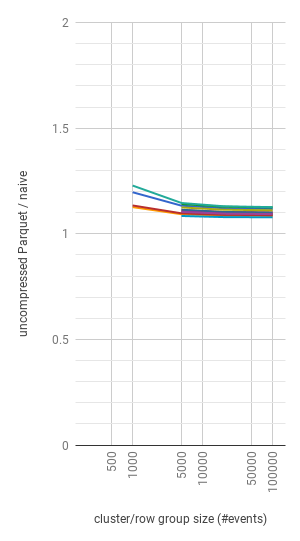
\includegraphics[width=\linewidth]{parquet-none.png}
\end{center}
\column{0.26\linewidth}
\begin{center}
ROOT gzip

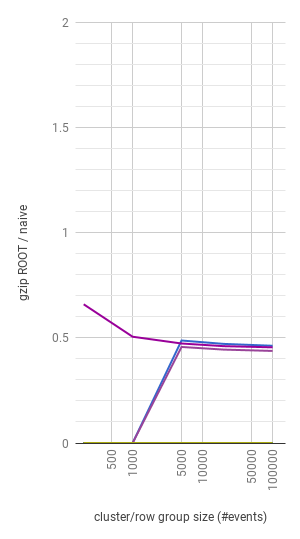
\includegraphics[width=\linewidth]{root-gzip.png}
\end{center}
\column{0.26\linewidth}
\begin{center}
Parquet gzip

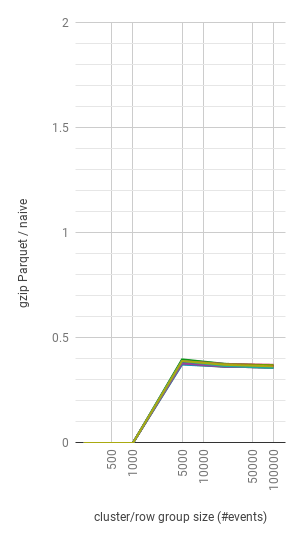
\includegraphics[width=\linewidth]{parquet-gzip.png}
\end{center}
\end{columns}

\vspace{0.25 cm}
Ensemble of 13 physics types vs.\ cluster size (ROOT) row group size (Parquet).
\end{frame}

\begin{frame}{But uncompressed$+$dictionary encoding is close to full gzip, lzma!}
\begin{columns}
\column{0.26\linewidth}
\begin{center}
\mbox{\hspace{3 cm}}
ROOT gzip

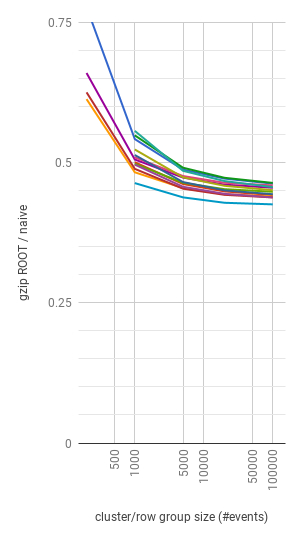
\includegraphics[width=\linewidth]{root-gzip-2.png}
\end{center}
\column{0.26\linewidth}
\begin{center}
\mbox{\hspace{3 cm}}
ROOT lzma

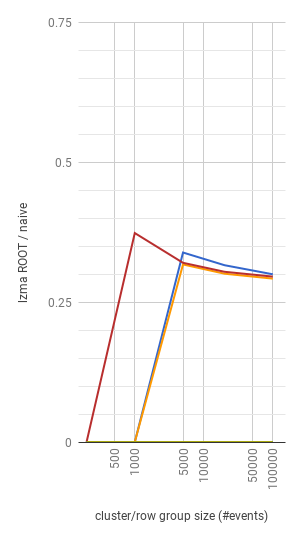
\includegraphics[width=\linewidth]{root-lzma.png}
\end{center}
\column{0.26\linewidth}
\begin{center}
\mbox{\hspace{3 cm}}
Parquet gzip

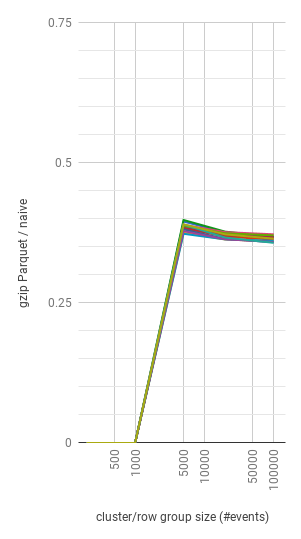
\includegraphics[width=\linewidth]{parquet-gzip-2.png}
\end{center}
\column{0.26\linewidth}
\begin{center}
Parquet uncompressed
with dict encoding

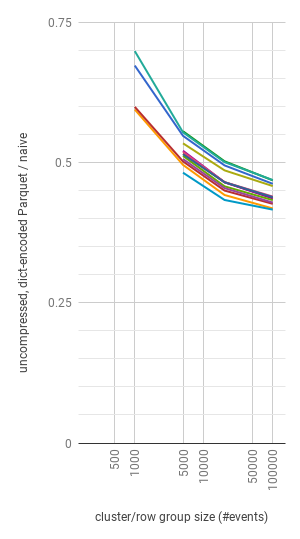
\includegraphics[width=\linewidth]{parquet-dict.png}
\end{center}
\end{columns}
\end{frame}

\begin{frame}{HERE}
\vspace{0.5 cm}
Highest cluster/row group (100\,000 events), total file size (sum of 13 physics types):

\begin{center}
\begin{tabular}{r c c | c c}
                    & \multicolumn{2}{c}{all branches} & \multicolumn{2}{c}{without trigger} \\
                    & ROOT & Parquet & ROOT & Parquet \\\hline
uncompressed        & \ldots & \ldots & \ldots & \ldots \\
dictionary encoding & & \ldots & & \ldots \\
lz4                 & \ldots & & \ldots & \\
gzip                & \ldots & \ldots & \ldots & \ldots \\
lzma                & \ldots & & \ldots & \\
\end{tabular}
\end{center}
\end{frame}



\end{document}
